\documentclass[titlepage]{jarticle}
\usepackage{h31ec-exp}
\usepackage[dvipdfmx]{graphicx}
\usepackage[yen]{okuverb}
\usepackage{here}

\title{光センサの使い方}
\grade{3年41番}%
\author{鷲尾 優作}
\team{A-3}
\date{令和3年7月5日,7月12日,7月19日}
\expdate{令和3年7月20日}
\coauthor{
  15番 & 小林 遼\\
  27番 & 滝沢 倖大\\
  %34番 & 西脇 光
}

\begin{document}
\maketitle

%目次の出力
\tableofcontents
\newpage

\section{実験背景}
\subsection{目的}
\begin{itemize}
    \item 制御システムにおいてフィードバックを行うため必要不可欠であるセンサについて学ぶ.
    \item 2種の光センサの特徴や特性を計測し、理解する.
    \item センサを活用する応用回路を自力で設計し、技術を身につける.
\end{itemize}

\subsection{光センサの選定方法}
光センサには様々な種類があり、目的に応じて適切に選定することが求められる.
重要な要素の代表例は、検出したい「波長」「必要な応答速度」である.

設計者はこれらを検討し、フォトダイオード、フォトトランジスタ、光導電素子、焦電素子、
光電管、カラーセンサ、CCDなどさまざまな種類の光センサから選び抜く力が求められる.

今回の実験では、課題として与えられた光導電素子(CdS)とフォトダイオードについて特性を測定する.

\section{各素子の構造及び原理}
\subsection{CdS光導電セル}
CdSは硫化カドミウムを主成分とした光導電素子で、照射光によって端子間電圧が変化する.
CdSは構造上応答速度が遅く、高速条件下でのスイッチングには不向きであるため
使用用途はゆるやかな照度変化の観測に限定される.
\subsection{フォトダイオード}
フォトダイオードは半導体のPN接合界面に光が入射すると電位差を生じる光起電力を利用している.
フォトダイオードは単体で起電力を有するため、外部の電源を必要とせず動作する.
このため電源がなくも簡単な光検出が可能であるが、その出力は極めて微弱なため、増幅回路を
併せて用いることが多い.
CdSと比較し2桁以上の高速応答性を持ち、入射光量と出力電流の直線性に優れる素子である.

\section{基礎特性測定}
LED光源をCdSセル、及びフォトダイオードに照射し、抵抗値・起電力の変化を観察する.
LEDに流れる電流とその光量は正比例しないため、ここでは光の強度によって変化する特性を
測定している.
\subsection{CdS光導電素子の特性}
以下図\ref{fig:CdS基礎特性評価回路}に実験回路図を示す.

\begin{figure}[H]
    \begin{center}
        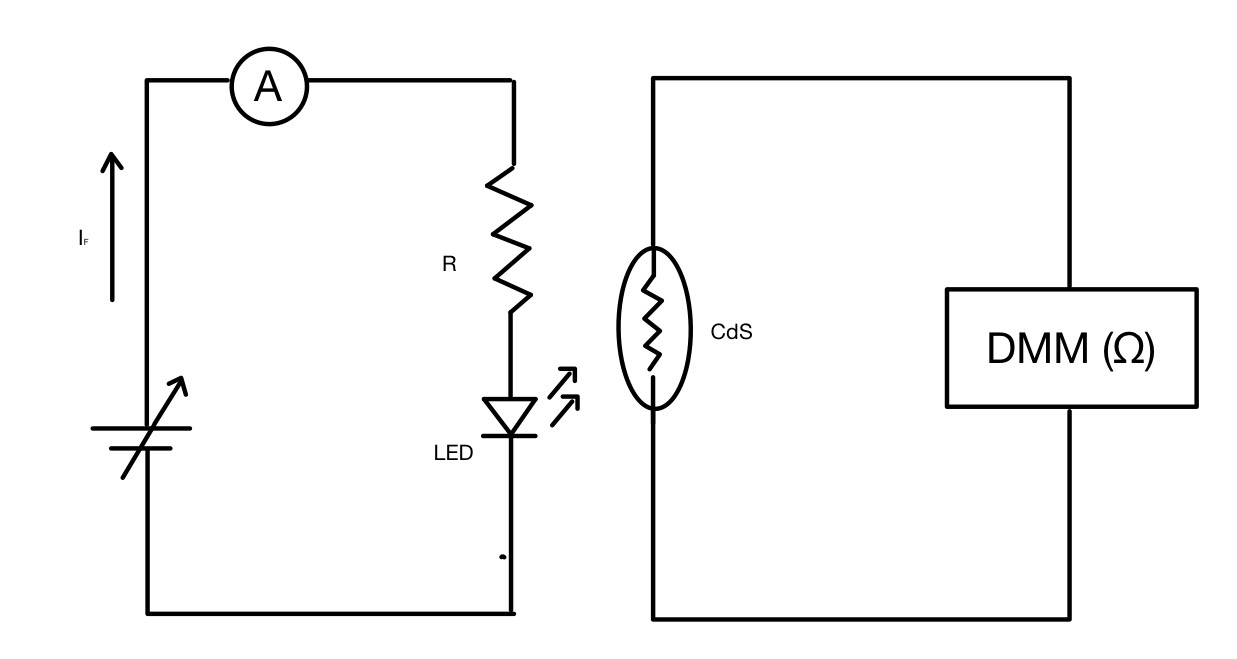
\includegraphics[width=10cm]{image/1.jpg}
        \caption{CdS基礎特性評価回路}
        \label{fig:CdS基礎特性評価回路}
    \end{center}
\end{figure}

\subsubsection{方法}
電源の電圧を0Vから徐々に上げ、LEDに流れる電流を増加させることで.
LEDに流れる電流は電流計で測定し、$I_F$=1mA,2mA,3mA...19mA,20mAと1mAづつ増加させる.
このときCdSの両端電圧をマルチメータで測定し光量-抵抗特性を測定する.

\subsubsection{使用器具}
\begin{enumerate}
    \item CdS光導電素子特性評価回路 CdS-A1 (MKY-54C348)
    \item 直流安定化電源装置 KIKUSUI PMC35-2 Ec-05
    \item デジタルマルチメータ SANWA CD770 EC-01
    \item 電流計 YOKOGAWA YAS1991
\end{enumerate}


以下表\ref{CdSセルの特性評価結果}に測定結果を表で示す.
\begin{table}[htbp]
    \begin{center}
        \caption{CdSセルの特性評価結果}
        \begin{tabular}{r|r}
            \hline\hline
            \multicolumn{1}{l|}{IF(mA)} & \multicolumn{1}{l}{Rc(Ω)} \\ \hline
            1                           & 2381                      \\ \hline
            2                           & 1517                      \\ \hline
            3                           & 1084                      \\ \hline
            4                           & 879                       \\ \hline
            5                           & 755                       \\ \hline
            6                           & 658                       \\ \hline
            7                           & 588                       \\ \hline
            8                           & 541                       \\ \hline
            9                           & 499                       \\ \hline
            10                          & 465                       \\ \hline
            11                          & 444.1                     \\ \hline
            12                          & 419.8                     \\ \hline
            13                          & 399.7                     \\ \hline
            14                          & 383.4                     \\ \hline
            15                          & 368.3                     \\ \hline
            16                          & 355.5                     \\ \hline
            17                          & 341.7                     \\ \hline
            18                          & 331.4                     \\ \hline
            19                          & 321.1                     \\ \hline
            20                          & 313.4                     \\ \hline
        \end{tabular}
        \label{CdSセルの特性評価結果}
    \end{center}
\end{table}

以下図\ref{fig:CdSセルの入射光と出力電圧の関係}に対数グラフを示す.
\begin{figure}[H]
    \begin{center}
        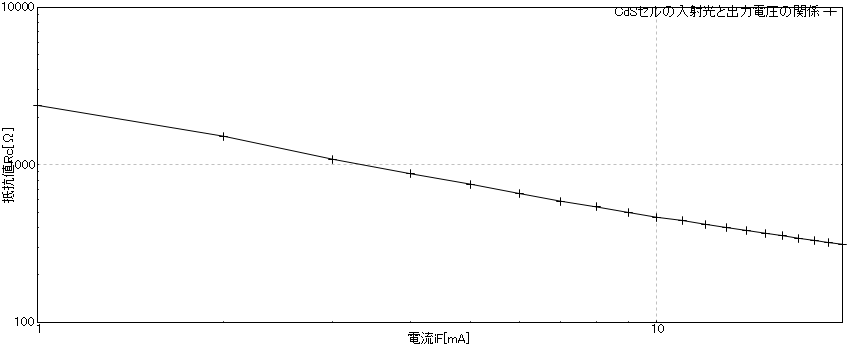
\includegraphics[width=10cm]{graph/1.PNG}
        \caption{CdSセルの入射光と出力電圧の関係}
        \label{fig:CdSセルの入射光と出力電圧の関係}
    \end{center}
\end{figure}

測定結果からは、光量に増加に伴って抵抗値が減少する特性がわかる.

\subsection{フォトダイオードの特性}
短絡特性、開放特性の2つについて測定する
\subsubsection{使用器具}
\begin{enumerate}
    \item フォトダイオード特性評価回路 PD-A5
    \item 直流安定化電源装置 KIKUSUI PMC35-2 Ec-05
    \item デジタルマルチメータ SANWA CD770 EC-10 Ec-17
    \item 電流計 YOKOGAWA YAS1991
    \item オシロスコープ GWINSTEK  GDS-1022 No.11
\end{enumerate}
\subsubsection{短絡特性の測定}
短絡特性はフォトダイオード両端子間を短絡させ、そのうえで入射光を与えた場合、
フォトダイオードの短絡電流はどのようになるかを測定するものである.

以下図\ref{fig:短絡特性評価回路}に実験回路を示す.

\begin{figure}[H]
    \begin{center}
        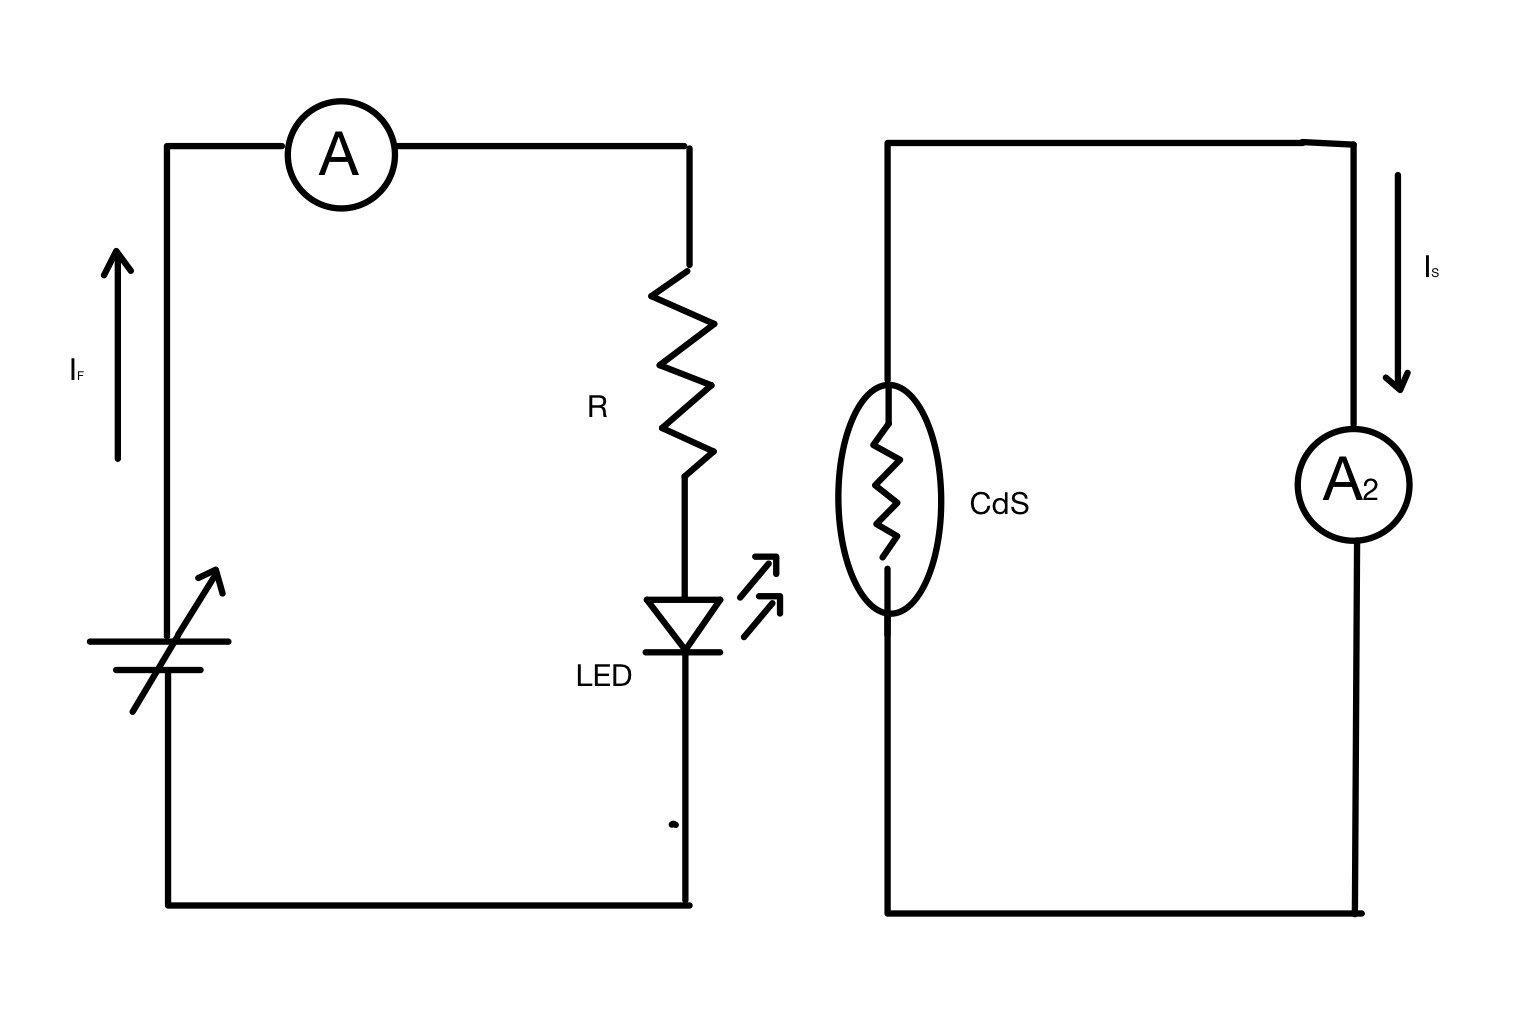
\includegraphics[width=10cm]{image/4.jpg}
        \caption{短絡特性評価回路}
        \label{fig:短絡特性評価回路}
    \end{center}
\end{figure}

CdS特性評価時と同様に入射光を発生させるLEDの電源電圧を0Vから徐々に上げ、LEDに流れる電流を増加させる.
LEDに流れる電流は電流計で測定し、$I_F$=1mA,2mA,3mA...19mA,20mAと1mAづつ増加させるものとする.
このときのフォトダイオードの短絡電流$I_S$を測定し表にまとめた.
結果は開放特性と併せて示す.

\subsubsection{開放特性の測定}
開放特性はフォトダイオード両端子間を開放し、そのうえで入射光を与えた場合、
フォトダイオードの両端に発生する起電力はどのようになるかを測定するものである.

以下図\ref{fig:開放特性評価回路}に実験回路を示す.

\begin{figure}[H]
    \begin{center}
        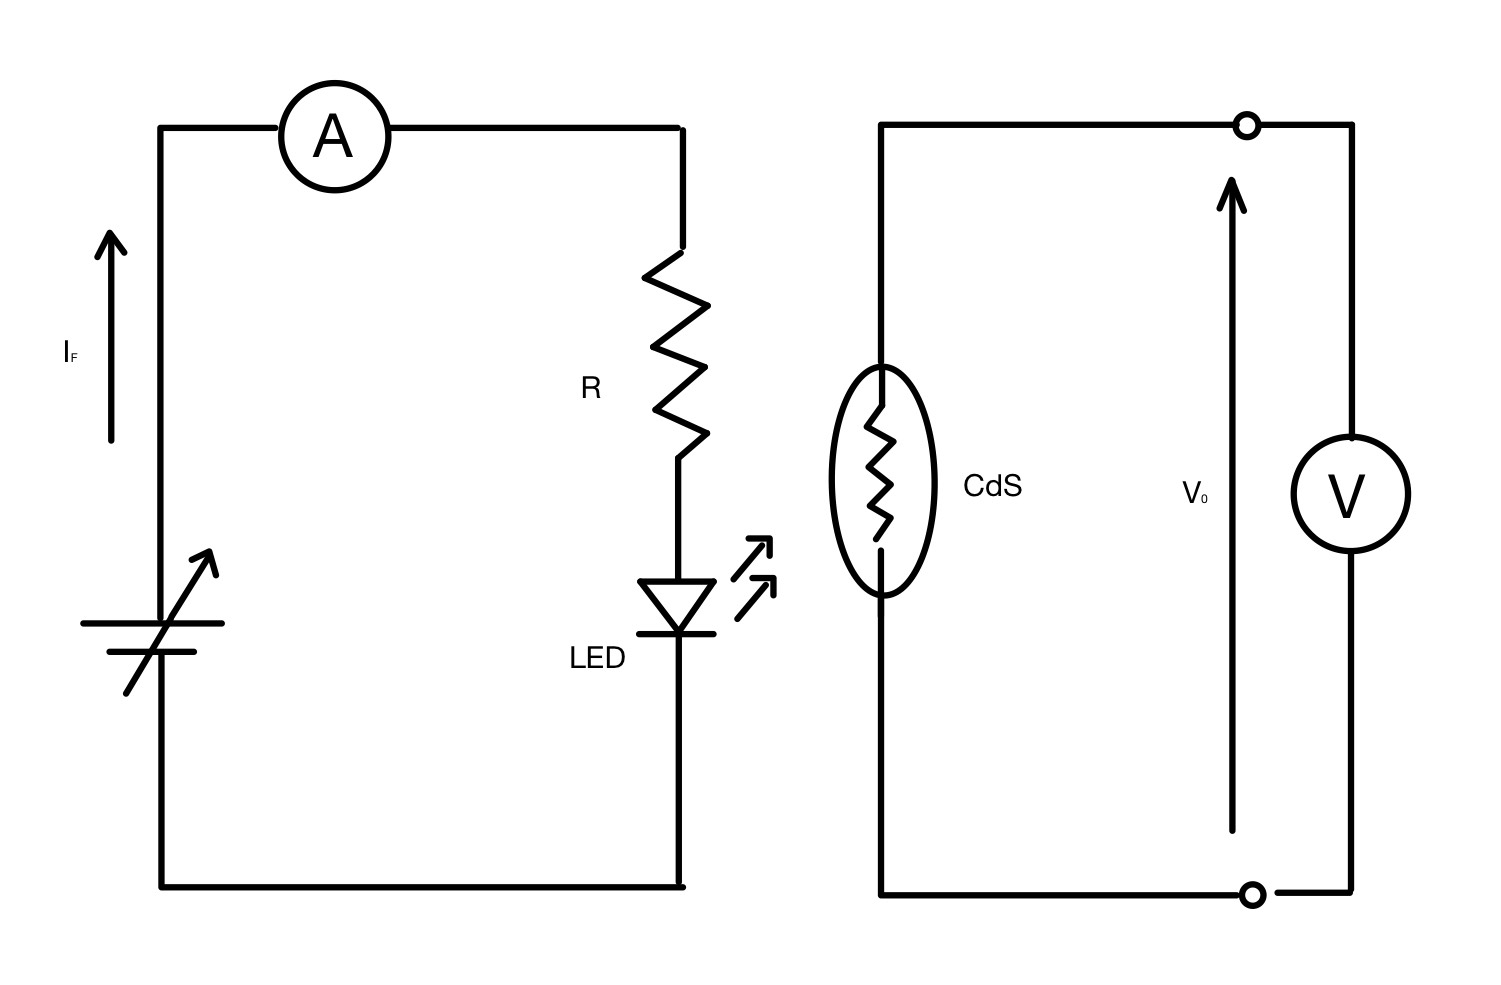
\includegraphics[width=10cm]{image/5.jpg}
        \caption{開放特性評価回路}
        \label{fig:開放特性評価回路}
    \end{center}
\end{figure}

前実験同様に入射光を発生させるLEDの電源電圧を0Vから徐々に上げ、LEDに流れる電流を増加させる.
LEDに流れる電流は電流計で測定し、$I_F$=1mA,2mA,3mA...19mA,20mAと1mAづつ増加させるものとする.
このときのフォトダイオードの開放電圧$V_0$を測定し表にまとめた.

以下表\ref{フォトダイオードの特性評価結果}に測定結果を示す.
\begin{table}[htbp]
    \begin{center}
        \caption{フォトダイオードの特性評価結果}
        \begin{tabular}{r|r|r}
            \hline\hline
            \multicolumn{1}{l|}{IF(mA)} & \multicolumn{1}{l|}{IS(uA)} & \multicolumn{1}{l}{V0[V]} \\ \hline
            5.0                         & 1.6                         & 0.400                     \\ \hline
            6.0                         & 2.0                         & 0.407                     \\ \hline
            7.0                         & 2.5                         & 0.412                     \\ \hline
            8.0                         & 2.9                         & 0.416                     \\ \hline
            9.0                         & 3.3                         & 0.419                     \\ \hline
            10.0                        & 3.8                         & 0.423                     \\ \hline
            11.0                        & 4.2                         & 0.425                     \\ \hline
            12.0                        & 4.6                         & 0.428                     \\ \hline
            13.0                        & 5.1                         & 0.430                     \\ \hline
            14.0                        & 5.5                         & 0.432                     \\ \hline
            15.0                        & 5.9                         & 0.434                     \\ \hline
            16.0                        & 6.3                         & 0.436                     \\ \hline
            17.0                        & 6.7                         & 0.438                     \\ \hline
            18.0                        & 7.1                         & 0.439                     \\ \hline
            19.0                        & 7.5                         & 0.441                     \\ \hline
            20.0                        & 7.9                         & 0.442                     \\ \hline
        \end{tabular}
        \label{フォトダイオードの特性評価結果}
    \end{center}
\end{table}

\newpage

以下図\ref{fig:フォトダイオードの短絡特性},\ref{fig:フォトダイオードの開放特性}にグラフを示す.
\begin{figure}[H]
    \begin{center}
        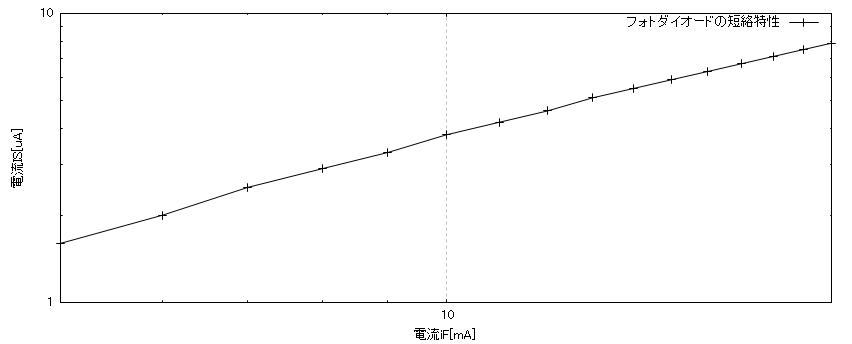
\includegraphics[width=10cm]{graph/2.PNG}
        \caption{フォトダイオードの短絡特性}
        \label{fig:フォトダイオードの短絡特性}
    \end{center}
\end{figure}

\begin{figure}[H]
    \begin{center}
        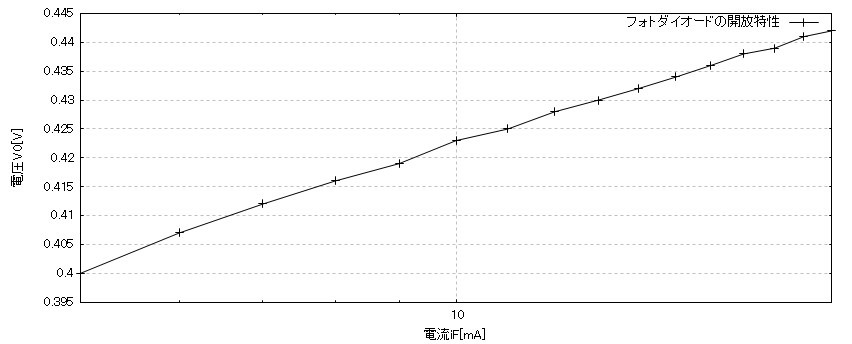
\includegraphics[width=10cm]{graph/3.PNG}
        \caption{フォトダイオードの開放特性}
        \label{fig:フォトダイオードの開放特性}
    \end{center}
\end{figure}

実験から、フォトダイオードは光量変化に対して電圧、電流の両要素について非常に直線的な性質をもっていることがわかる.
CdSと異なり、フォトダイオードは光量の増加に対して抵抗値が増す特性をもつこともわかる.

\section{CdSを用いた回路の作成}
\subsection{明暗判定回路の作成}
CdSを用いて、暗いと判定した場合赤色LEDが点灯する回路を作成する.

以下図\ref{fig:明暗判定回路図}に回路図を示す.
\begin{figure}[H]
    \begin{center}
        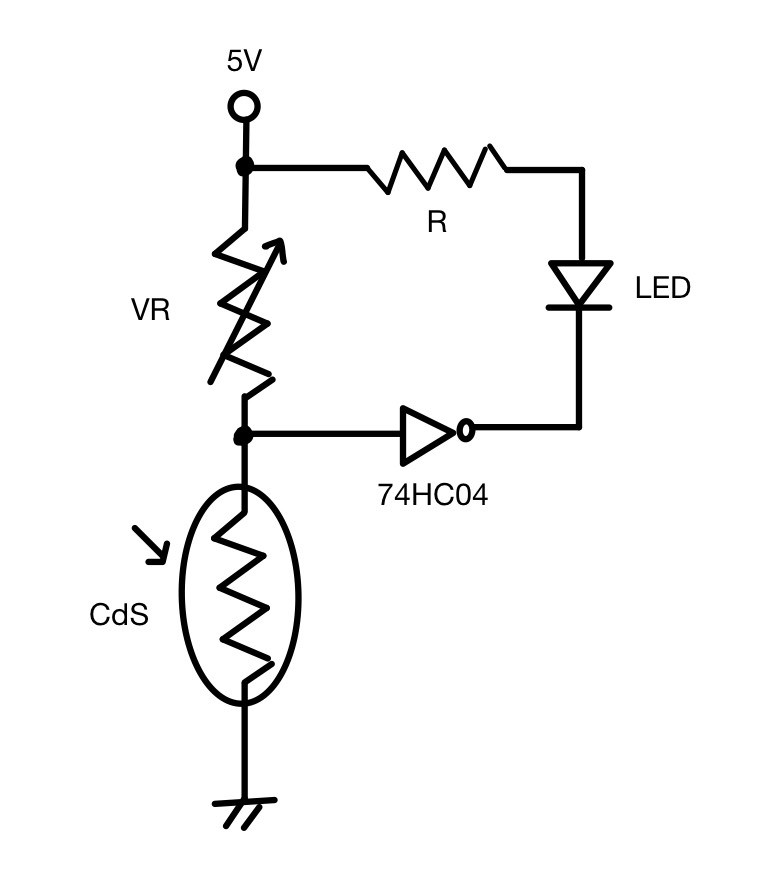
\includegraphics[width=10cm]{image/2.jpg}
        \caption{明暗判定回路図}
        \label{fig:明暗判定回路図}
    \end{center}
\end{figure}

使用した素子は以下である
\begin{enumerate}
    \item CdS MKY-54C348
    \item 赤色LED L-513LE1T
    \item インバータIC 74HC04
\end{enumerate}

動作原理は次のとおりである.

CdSは暗くなるほど抵抗値が増す.したがって
$VR*CdS/VR+CdS$で示されるインバータICの入力端子の電位は、
分圧則に従い、明るいほど0Vに近く、暗いほど5Vに近くなる.

この電位がインバータICの入力閾値に対して高いか低いかでインバータの入力が決定される
暗い場合、インバータの入力はHIGH(1)となり出力はLOW(0)となる.
このときLEDの両端には電位差が生じているため、LEDは点灯する.
また同様に、明るい場合インバータの入力はLOW(1)となり出力はHIGH(1)
であるので、LED両端は1-1で電位差が存在せず、消灯する.

明暗の点灯の閾値は半固定抵抗$VR$の抵抗値を操作することで変更可能である.

\subsection{応用回路の設計製作}
前項目の判定回路を参考にし、明るい場合緑LEDを、暗い場合赤LEDを点灯させる
応用回路を設計する.

以下図\ref{fig:応用回路回路図}に設計した応用回路を示す.
\begin{figure}[H]
    \begin{center}
        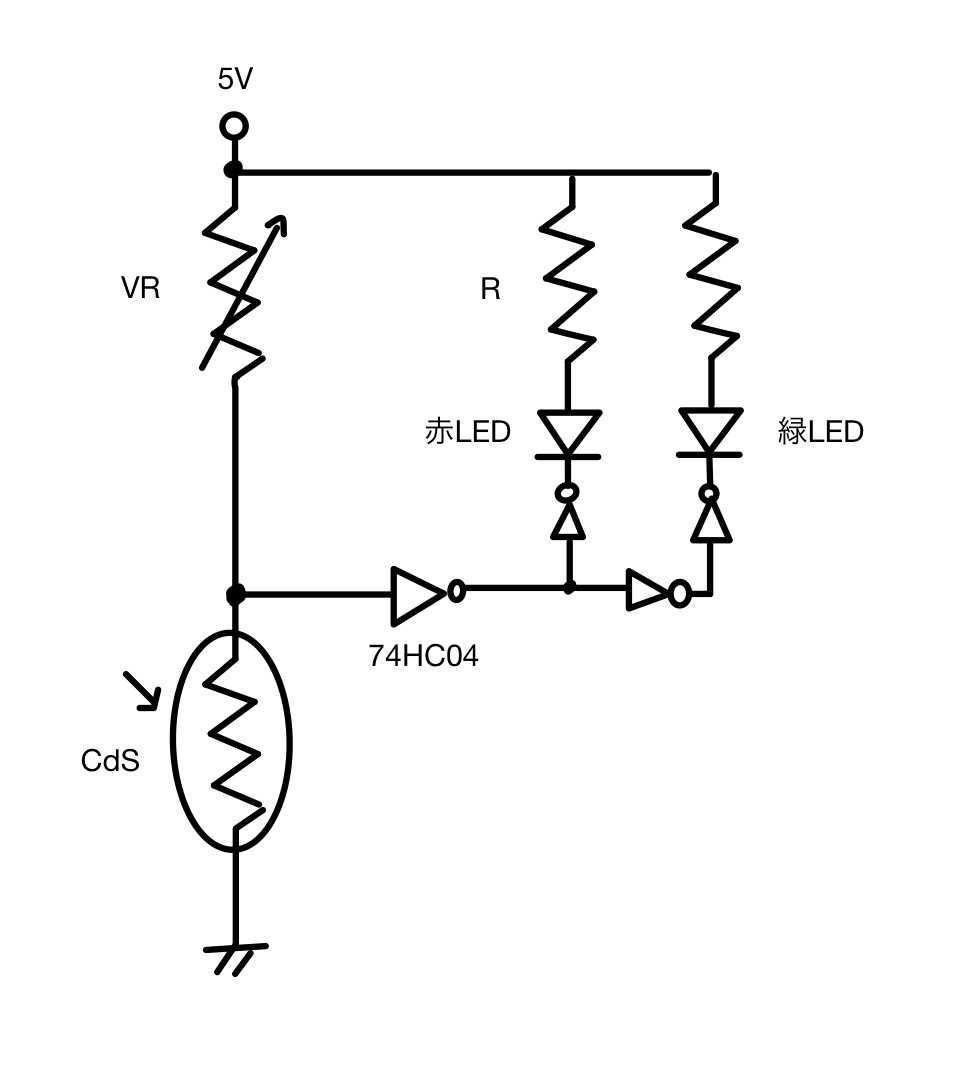
\includegraphics[width=10cm]{image/3.jpg}
        \caption{応用回路回路図}
        \label{fig:応用回路回路図}
    \end{center}
\end{figure}

前項目に加え、以下の部品を使用した
\begin{enumerate}
    \item 緑色LED L-513SGT3
    \item 半固定抵抗 10kΩ
    \item 炭素被膜抵抗 1kΩ * 2
\end{enumerate}

以下に設計した回路を示す.
赤色LEDと緑色LEDは並列に接続されており、判定用インバータの出力0,1に対して、
赤色LEDは二重反転、緑色LEDは一重反転とすることで
同時に点灯しないように設計している.
判定インバータの出力は暗い場合にLOW(0)となるので、このとき緑色LEDは消灯
赤色LEDは点灯する.

なお赤色LEDを直接接続でなく二重反転としているのはLEDに流れる電流をデジタル的に
制御し安定させるためである.

\section{フォトダイオードとオペアンプを利用した照度計の作成}
フォトダイオードの出力をオペアンプによって増幅し照度計として利用する方法を学ぶ.
回路に光を照射しその挙動を観察した.

以下図\ref{fig:照度系内部回路}に回路を示す.
\begin{figure}[H]
    \begin{center}
        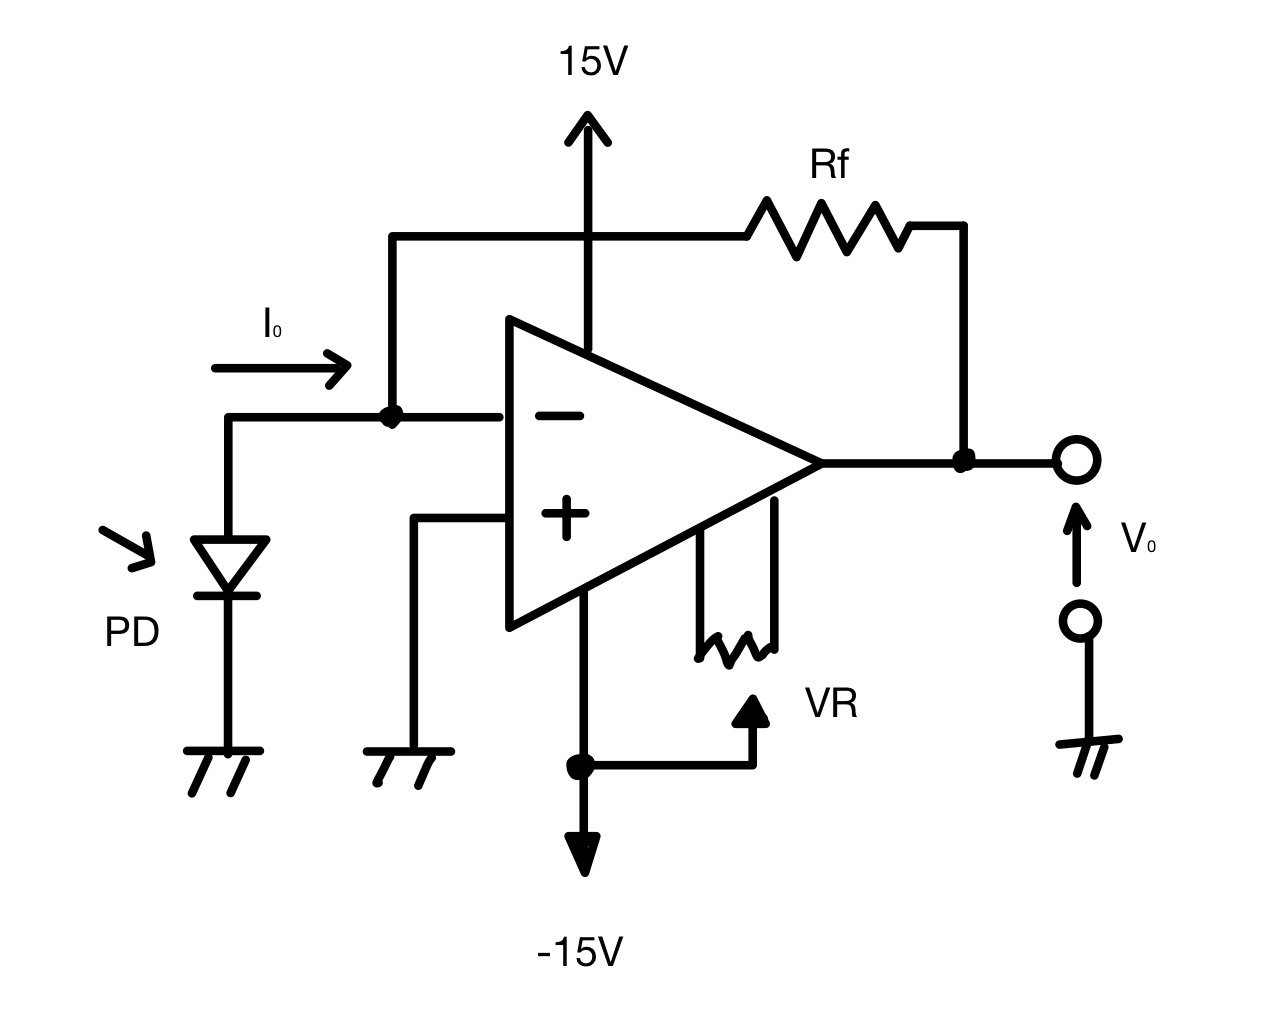
\includegraphics[width=10cm]{image/6.jpg}
        \caption{照度計内部回路}
        \label{fig:照度系内部回路}
    \end{center}
\end{figure}

以下に実験回路図を示す.
この回路を作成するにあたっては、オペアンプとフォトダイオード間の配線を
できるだけ短くするよう配慮する必要がある.

また、この回路を用いて蛍光灯の光を照射したときの出力電圧$V_0$をオシロスコープで観測した.

以下図\ref{オシロスコープ画像}に出力した画像を示す.
\begin{figure}[H]
    \begin{center}
        \includegraphics[width=10cm]{image/A0000DS.BMP}
        \caption{オシロスコープ画像}
        \label{オシロスコープ画像}
    \end{center}
\end{figure}
周波数52.9[kHz]、周期は18.9[us]であること、またそれを正弦波に近く観察できるような高速応答性をフォトダイオードが
備えていることがわかる.

\section{考察}
CdS、フォトダイオード間には明確な特性の差があることがわかった.
全体的にフォトダイオードであればCdSの使用目的をほぼ満たせると考えられる.
ただし、今回CdSの応答性の測定等を行っていないため、実験としては不十分と思われる.
金銭的な問題がなければフォとダイオードを剪定することが望ましいと現時点では考える.

\section{課題}
\subsection{課題1}
CdSは、街路灯、夜間の保安灯、車のオートライトなど、ミサイルの熱誘導などに用いられる.
無極性、耐電圧の高さ、電流電圧特性が比例的である等利用が簡単であるため、幅広く用いられている.
\subsection{課題2}
CDプレーヤーやテレビのリモコン、ビデオテープレコーダー等に使用される.
医療用器具の断層X線写真機等などにも使用され、高速で明滅する光信号の受信用途に用いられることが多い.
\subsection{課題3}
フォトトランジスタはフォトダイオードとトランジスタを組み合わせたもので、出力がhFE倍される素子である。
このためフォトトランジスタにみられる出力が小さいという不利に対応できる。
フォトトランジスタの数百倍の出力を持ち、数Luxで動作する。
使用用途は一般的にフォトダイオードと同様の分野である.

\begin{thebibliography}{99}
    \bibitem{}「光センサの使い方,令和3年度電子制御工学実験・3年前期テキスト」
    \bibitem{} 3分でわかる技術の超キホン https://engineer-education.com
    \bibitem{} コーデンシ https://www.kodenshi.co.jp
\end{thebibliography}

\end{document}